%%
%% Copyright (C) Hochschule Esslingen, 2011
%%
%% $Id: example.tex 131 2011-10-16 01:11:22Z uwe $
%%
%% This work may be distributed and/or modified under the
%% conditions of the LaTeX Project Public License, either version 1.3
%% of this license or (at your option) any later version.
%% The latest version of this license is in
%%   http://www.latex-project.org/lppl.txt
%% and version 1.3 or later is part of all distributions of LaTeX
%% version 2005/12/01 or later.


\begin{document}

% If you wish to uncover everything in a step-wise fashion, uncomment
% the following command: 
% \beamerdefaultoverlayspecification{<+->}

\mode<article>{\maketitle}

\begin{frame}
  \titlepage
\end{frame}

\begin{frame}{Content}
  \tableofcontents
\end{frame}

\section{Introduction}

\subsection{Die Dateien}

\begin{frame}[fragile]{Das Theme Esslingen für Beamer-Präsentationen}
Zum Paket gehören die folgenden Dateien:

\rowcolors{1}{HEblue4}{HEblue2}

\begin{center}
  \begin{tabular}{lp{6cm}}
    beamercolorthemeEsslingen.sty & Farbdefinitionen \\
    beamerfontthemeEsslingen.sty & Schriftauswahl \\
    beamerouterthemeEsslingen.sty & Kopf-, Fußzeile, Logo, Seitentitel\\
    beamerthemeEsslingen.sty & weitere Definitionen \\
    Esslingen-Defs.sty & die Farbdefinitionen zum Einbinden in \LaTeX-Dateien.\\
  \end{tabular}
\end{center}
Aufgerufen wird das Theme Esslingen in der Präambel mittels
\verb+\usetheme{Esslingen}+

\end{frame}

\begin{frame}{Abbildungen} 
Im Ordner \texttt{figures} befinden sich die folgenden Bilder im eps- und
png-Format sowie eine avi-Animation.

\rowcolors{1}{HEblue4}{HEblue2}
\begin{center}
  \begin{tabular}{lp{6cm}}
  HEGoeppingen & Das Hochschulgebäude \\
  HEGrid & Das Grid (Titelseite rechts oben) \\
  HELogo & Das Logo der Hochschule Esslingen \\
  TubeKnot & Das Standbild der Knoten-Animation \\
  TubeKnot.avi & Eine kurze Animation eines Knotens \\
  \end{tabular}
\end{center}

Die Bilder \texttt{HELogo}, \texttt{HEGoeppingen} und \texttt{HEGrid} werden
für die Titelseite benutzt. \texttt{HELogo} erscheint außerdem in jeder
Titelzeile eines Frames.

\end{frame}

\begin{frame}[fragile]{Die Beispiel-Datei}
Es liegt eine Beispiel-Datei in drei Formen bei. 
\rowcolors{1}{HEblue4}{HEblue2}
\begin{center}
  \begin{tabular}{lp{6cm}}
    example-beamer.tex &  die Beamer-Präsentation \\
    example-handout.tex & A4-Handout der Beamer-Frames \\
    example-article.tex & Article-Handout \\
  \end{tabular}
\end{center}

Die drei PDF-Dateien können entweder gemeinsam über das beiliegende make-File
oder einzeln mit den Befehlen
\begin{verbatim}
  pdflatex example-beamer.tex
  pdflatex example-handout.tex
  pdflatex example-article.tex
\end{verbatim}
erzeugt werden. Die drei LaTex-Dateien binden jeweils die Dateien
\texttt{preamble.tex} und \texttt{example.tex} ein.

\end{frame}

\section{Layout-Elemente}

\begin{frame}[fragile]{Die Fußzeile}
  \begin{itemize}
  \item Die Einträge in der Fußzeile werden aus den optionalen Argumenten der
  Befehle \texttt{title}, \texttt{subtitle}, \texttt{author},
  \texttt{\institute} und \texttt{date} in der Titelseite
  zusammengesetzt. 

  \item Die Fußzeile kann zwischen den Frames mit dem Befehl
\begin{verbatim}
   \setbeamertemplate{footline}{}
\end{verbatim}
für die nachfolgenden Frames ausgeschaltet werden. Dadurch gewinnt man etwas
Platz auf der Seite.
  \end{itemize}
\end{frame}

% Ausschalten der Fußzeile
\setbeamertemplate{footline}{}

\subsection{Die Farbtabelle}

\begin{frame}{Die Farbtabelle}
\label{frame:Farbtabelle}
\begin{table}[h]
    \centering
    \caption{Vordefinierte Farben entsprechend Corporate Design}
      \begin{tabular}{clll}
        \toprule
        \textbf{Farbe} & \textbf{Kürzel} & \textbf{RGB-Wert} & \textbf{Verwendungsbeispiel} \\
        \midrule
        \color{HEblue6}\rule{30pt}{8pt} & HEblue6 &    0,   70,  102 & Überschriften \\
        \color{HEblue5}\rule{30pt}{8pt} & HEblue5 &   85,  146,  172 &  \\
        \color{HEblue4}\rule{30pt}{8pt} & HEblue4 &  168,  203,  221 & Hauptüberschriften \\
        \color{HEblue3}\rule{30pt}{8pt} & HEblue3 &  206,  226,  236 &  \\
        \color{HEblue2}\rule{30pt}{8pt} & HEblue2 &  236,  242,  245 &  \\
        \color{HEblue1}\rule{30pt}{8pt} & HEblue1 &  245,  248,  249 & Abbildungshintergrund \\
        \color{HEgray1}\rule{30pt}{8pt} & HEgray1 &  112,  113,  114 & Aufzählungszeichen \\
        \color{HEred2}\rule{30pt}{8pt}  & HEred2  &  212,    0,   50 & Überschriften, Logo \\
        \color{HEred1}\rule{30pt}{8pt}  & HEred1  &  230,  143,  126 &  \\
        \bottomrule
      \end{tabular}
  \end{table}
\end{frame}

% 
\mode<article>{
\begin{figure}[h]
  \centering
  \fbox{\includeslide[height=5cm]{frame:Farbtabelle}}
  \caption{Bildimport aus der Präsentationsdatei.}
  \label{fig:slide.farbtabelle}
\end{figure}
}

\begin{frame}[fragile]{Die Fußzeile}
  Mit dem Befehl
\begin{verbatim}
  \setbeamertemplate{footline}[Esslingen theme]
\end{verbatim}
  wird die Fußzeile wieder auf die voreingestellte Variante zurückgesetzt.
\end{frame}

% Wiedereinschalten der Fußzeile
\setbeamertemplate{footline}[Esslingen theme]

\subsection{Listen}

\begin{frame}{Itemize-, Enumerate- und Description-Listen}

Die Itemize-Liste
    \begin{itemize}
      \item Erste Ebene.
       \begin{itemize}
        \item Zweite Ebene.
       \end{itemize}
    \end{itemize}

Die Enumerate-Liste
  \begin{enumerate}
   \item Erster Eintrag
    \begin{enumerate}
     \item Erster Eintrag, zweite Ebene
    \end{enumerate}
  \end{enumerate}

Die Description-Liste
  \begin{description}
  \item[Eintrag] Erläuterung
  \end{description}

\end{frame}

\begin{frame}{Anpassung der Listen-Items}
Das Layout der Zähler und Listen-Items lässt sich leicht anpassen. Diese
Möglichkeit sollte aber nur zurückhaltend genutzt werden.

\setbeamertemplate{itemize item}{\Large\guillemotright}
\setbeamertemplate{itemize subitem}{--}
\setbeamertemplate{itemize subsubitem}{\textbullet}

\begin{itemize}
   \item Erste Ebene.
       \begin{itemize}
        \item Zweite Ebene.
       \begin{itemize}
        \item Dritte Ebene.
       \end{itemize}
       \end{itemize}
\end{itemize}
\begin{enumerate}[1.]
  \item Erster Eintrag
  \begin{enumerate}[(i)]
  \item Erster Eintrag, zweite Ebene
  \begin{enumerate}[a)]
  \item Erster Eintrag, dritte Ebene
  \end{enumerate}
  \end{enumerate}
\end{enumerate}
\end{frame}

\subsection{Blöcke}

\begin{frame}[fragile]{Blöcke}
Ob die Blöcke mit farbigem Hintergrund ausgegeben werden und wie kräftig
dieser ist, kann mit den folgenden Color-Themes in der Datei preamble.text 
gesteuert werden. (Voreingestellt ist \texttt{rose}.)

  \begin{itemize}
  \item \begin{verbatim}% \usecolortheme{lily}% kein Farb-Hintergrund\end{verbatim}
  \item \begin{verbatim}\usecolortheme{rose}% dezenter Farb-Hintergrund\end{verbatim}
  \item \begin{verbatim}% \usecolortheme{orchid}% kräftiger Farb-Hintergrund\end{verbatim}
  \end{itemize}
  \begin{block}{Überschrift}
    Ein Block.
  \end{block}
  \begin{alertblock}{Überschrift}
    Ein Alert-Block.
  \end{alertblock}
  \begin{example}
    Ein Beispiel-Block.
  \end{example}
\end{frame}

\begin{frame}{Satz und Beweis}
  \begin{theorem}%[Ein Satz mit Namen]
    Lorem ipsum dolor sit amet, consetetur sadipscing elitr, sed diam nonumy
    eirmod tempor invidunt ut labore et dolore magna aliquyam erat, sed diam
    \begin{equation}
      \label{eq:Satz}
      \sum_{i=1}^{\infty}\frac{1}{x^2}
    \end{equation}
  \end{theorem}
  \begin{proof}%[Der Beweis eines benannten Satzes]
    Lorem ipsum dolor sit amet, consetetur sadipscing elitr, sed diam nonumy
    eirmod tempor invidunt ut labore et dolore magna aliquyam erat, sed diam
    voluptua. At vero eos et accusam et justo duo dolores et ea rebum. Stet
    clita kasd gubergren, no sea takimata sanctus est Lorem ipsum dolor sit
    amet. 
  \end{proof}
\end{frame}

\begin{frame}[fragile]{Listings}
Quellcode-Listings lassen sich in-line \lstinline|print "hello world"| und in
der lstlisting-Umgebung des Pakets listing.sty darstellen.

\begin{lstlisting}[frame=single, emph={cout}, emphstyle={\color{blue}}]
   cout << "Hello world!";
\end{lstlisting}
\end{frame}

\begin{frame}[fragile]{Java}
huuhu
\begin{lstlisting}[frame=single]
   import com.aurel.track;

 public class TestClass {
    private String dummy;
 }
   cout << "Hello world!";
\end{lstlisting}
\end{frame}

\subsection{Animationen}

\begin{frame}{Animationen}{Einbindung mit dem Paket multimedia.sty}
Wie und ob Animationen angezeigt werden, ist abhängig vom Betriebssystem und
vom PDF-Betrachter.

\begin{columns}
  \column{.5\textwidth}
Klicken Sie auf das Bild, um die Animation mit einem externen Betrachter anzuzeigen.
  \column{.45\textwidth}
  \movie[externalviewer]{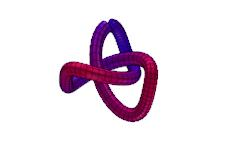
\includegraphics[scale=.5]{figures/TubeKnot}}{figures/TubeKnot.avi}
\end{columns}
\end{frame}




\begin{frame}{Zum Schluss}
  \begin{center}
    {\Huge \textcolor{HEblue6}{\bf Happy \LaTeX{}-ing!}}
  \end{center}
\end{frame}



\section{Literaturverzeichnis}

\begin{frame}
    \frametitle{Literaturverzeichnis}
  \begin{thebibliography}{9}

  \beamertemplatearticlebibitems

  \bibitem{Farbtabelle}
    \textit{Richtlinien für die Anfertigung von Seminar-, Bachelor- und
    Masterarbeiten}

    \newblock{Fakultät Betriebswirtschaft; Hochschule Esslingen; Flandernstraße 101; 73732 Esslingen}

  \bibitem{LaTeX Beamer class development repository}
    \textit{LaTeX Beamer class development repository.}
    \newblock{\url{https://bitbucket.org/rivanvx/beamer/wiki/Home}}

  \bibitem{beameruserguide}
    Till Tantau, Joseph Wright, and Vedran Mileti\'c
   \newblock{\textit{The beamer class --
    User Guide for version 3.10.}}
    \newblock{\url{http://www.ctan.org/tex-archive/macros/latex/contrib/beamer/doc/beameruserguide.pdf}}
  \end{thebibliography}

\end{frame}
\end{document}
